% inicia os apêndices

\begin{apendicesenv}

\chapter{Saídas auxiliares}

\begin{figure}[hbtp]
	\centering
	\caption{Verificação de quebras estruturais: OLS-CUSUM VAR($2$)} \label{figure:ols_cusum_model2}
	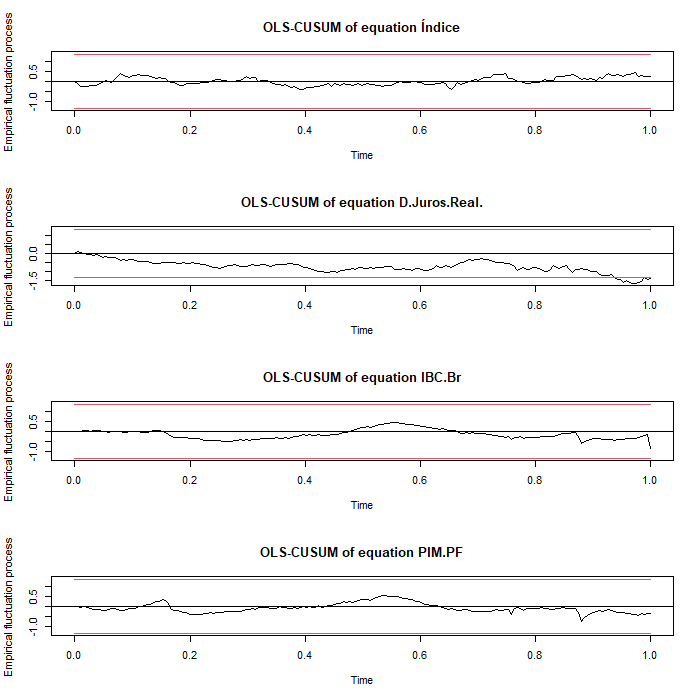
\includegraphics[scale = 0.90]{figuras/ols_cusum_model2.png}
	\fonte{Elaboração do autor.}
\end{figure}

\begin{table}[hbtp]
	\centering
	\caption{Raízes do polinômio característico do VAR($2$)} \label{table:raizes_var_2}
	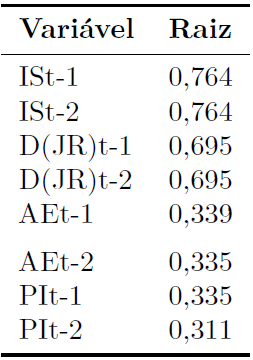
\includegraphics[scale = 0.50]{figuras/raizes_polinomio_caracteristico.PNG}
	\fonte{Elaboração do autor.}
\end{table}

\begin{table}[hbtp]
	\centering
	\caption{Coeficientes da equação do índice de sentimentos do VAR($2$)} \label{table:coef_IS_var_2}
	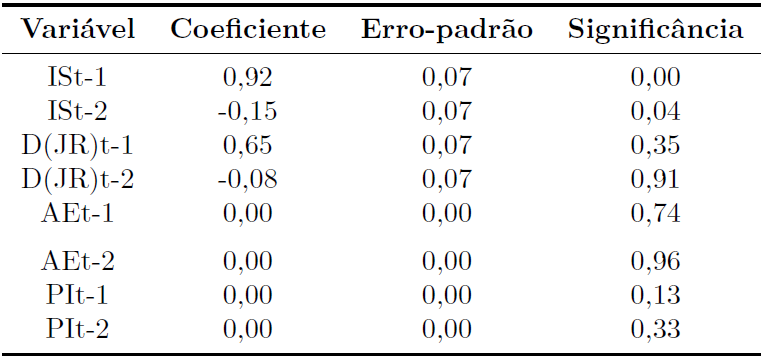
\includegraphics[scale = 0.50]{figuras/coeficientes_IS_var_2.PNG}
	\fonte{Elaboração do autor.}
\end{table}

\begin{table}[hbtp]
	\centering
	\caption{Coeficientes da equação da diferença da taxa de juros real do VAR($2$)} \label{table:coef_JR_var_2}
	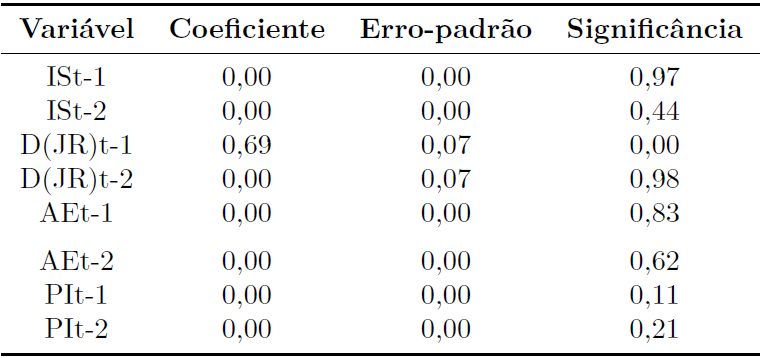
\includegraphics[scale = 0.50]{figuras/coeficientes_JR_var_2.PNG}
	\fonte{Elaboração do autor.}
\end{table}

\begin{table}[hbtp]
	\centering
	\caption{Coeficientes da equação da atividade econômica do VAR($2$)} \label{table:coef_AE_var_2}
	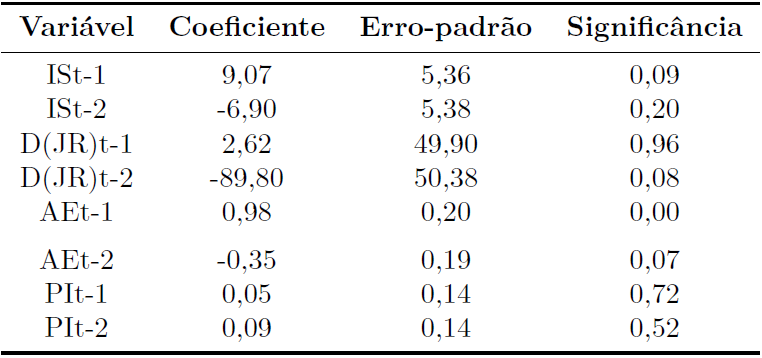
\includegraphics[scale = 0.50]{figuras/coeficientes_AE_var_2.PNG}
	\fonte{Elaboração do autor.}
\end{table}

\begin{table}[hbtp]
	\centering
	\caption{Coeficientes da equação da produção industrial do VAR($2$)} \label{table:coef_PI_var_2}
	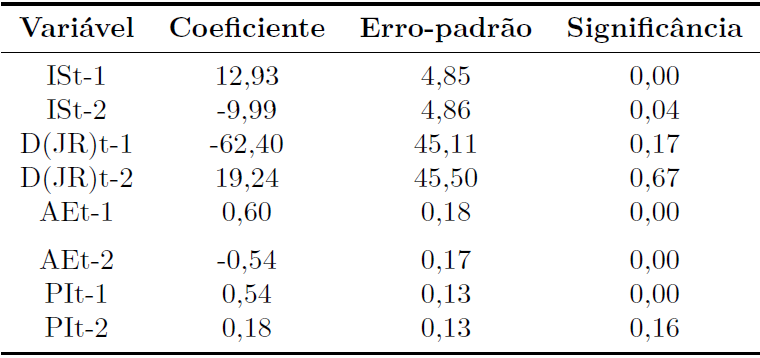
\includegraphics[scale = 0.50]{figuras/coeficientes_PI_var_2.PNG}
	\fonte{Elaboração do autor.}
\end{table}

\chapter{Códigos}

Todos os códigos utilizados no presente trabalho estão disponíveis no repositório online dessa monografia, sendo possível ser acessado por meio deste \href{https://github.com/cairebarletta/tcc}{link}.

\end{apendicesenv}
